\documentclass[12pt,letterpaper]{article}
\usepackage[latin1]{inputenc}
\usepackage{amsmath}
\usepackage{amsfonts}
\usepackage{amssymb}
\usepackage{graphicx}
%\usepackage{caption}
%\usepackage{gensymb}
\graphicspath{{./plots/}}
\begin{document}
{\centering
\title{Growing Degree Day Project \\ \vspace{.5 cm} {\Large Computer Based and Application Tools Course Project} }
\maketitle
%\author{Ozair Shafiq ~ Farhad M. Kazemi ~ Yeni Liang ~ Minhaj Shunjaruff \\ Zahed khatooni ~  Silvana Pereira ~  Ibrahim Alonge}

{\itshape Memorial University of Newfoundland \\ St. John's, Canada.\par}
}
\begin{abstract}
Growing degree days (GDD), also called growing degree units (GDUs), are a heuristic tool in phenology. GDD are a measure of heat accumulation used by horticulturists, gardeners, and farmers to predict plant and animal development rates such as the date that a flower will bloom, or a crop will reach maturity.
\\
The aim of this research is to find the...
\\The results showed that...
\end{abstract}

\section{Introduction}
In the absence of extreme conditions such as unseasonal drought or disease, plants grow in a cumulative stepwise manner which is strongly influenced by the ambient temperature. Growing degree days take aspects of local weather into account and allow gardeners to predict (or, in greenhouses, even to control) the plants' pace toward maturity.\\
Unless stressed by other environmental factors like moisture, the development rate from emergence to maturity for many plants depends upon the daily air temperature. Because many developmental events of plants and insects depend on the accumulation of specific quantities of heat, it is possible to predict when these events should occur during a growing season regardless of differences in temperatures from year to year. Growing degrees (GDs) is defined as the number of temperature degrees above a certain threshold base temperature, which varies among crop species. The base temperature is that temperature below which plant growth is zero. GDs are calculated each day as maximum temperature plus the minimum temperature divided by 2 (or the mean temperature), minus the base temperature. GDUs are accumulated by adding each day's GDs contribution as the season progresses.\\
GDUs can be used to: assess the suitability of a region for production of a particular crop; estimate the growth-stages of crops, weeds or even life stages of insects; predict maturity and cutting dates of forage crops; predict best timing of fertilizer or pesticide application; estimate the heat stress on crops; plan spacing of planting dates to produce separate harvest dates. Crop specific indices that employ separate equations for the influence of the daily minimum (nighttime) and the maximum (daytime) temperatures on growth are called crop heat units (CHUs).
\\
In this report, we would like to...
\\
\begin{equation}
\textrm{GDD} = \left(\frac{T_{max} + T_{min}}{2}\right) - T_{base}
\label{eqn:gdd}
\end{equation}
\\
On the rest of this report, firstly we will describe our dataset properties and what we have done to clean this data and to overcome data heterogeneity and missing values. In the second section, we briefly described ....
Finally, we have a conclusion and what could be done in the future works.
\section{Question 1:Dealing With Dataset}
Prerequisite of this script is a text file that will contain two strings separated by a comma on each line. The left string specifies the station name or its sub-name, the right string specifies the province that this station may belong to. The script takes the left string and searches it in Station Inventory EN file at Historical Climate data service provided by the government of Canada. It will fetch daily temperatures for stations that either match completely with the left string or sub-matches with the left string. For example, if the left string is 'toronto', all stations names in Station Inventory EN that contain the string 'toronto' will be matched by the script  and if the data is available for the specific years asked by the user, then its daily data for each of those years will be downloaded. The script will then combine all this data, sort the data date-wise and write this to a '/data' folder for convenience, for each line in the text file.\\
The program will also generate another text file that will contain the latitudes and longitudes for each location specified in the input text as the coordinates of that station that occupies the most years in the requested time-line.\\
Hence, the program requires two command line arguments, a text file containing station name, province pair in each line and Year specified as 'yyyy' that specifies the time-line as 2016-Year. For example, if 2012 is provided as the year, the program will fetch data for 2012 till 2016 time-line.

\section{Question 2}
This programs depends on data downloaded by core task 1, i.e. download.py. It reads the city name available in cities.txt and try to locate the city's csv file in download folder. Once located it fetches minimum and maximum temperature for every city and for all the years mentioned in the csv files. After that, based on the argument provided it plots the minimum and maximum temperature plot for every city in cities.txt file and for the year chosen.\\
Ex-\\
           python MinMax.py cities.txt 2010\\
will plot the min or max temp for year 2010 for the cities given in cities.txt file as below.
\begin{figure}
\centering
\includegraphics[scale=0.6]{{"st. john's,newfoundland_MinMax"}.png}
%\caption{D}
\end{figure}

\begin{figure}
\centering
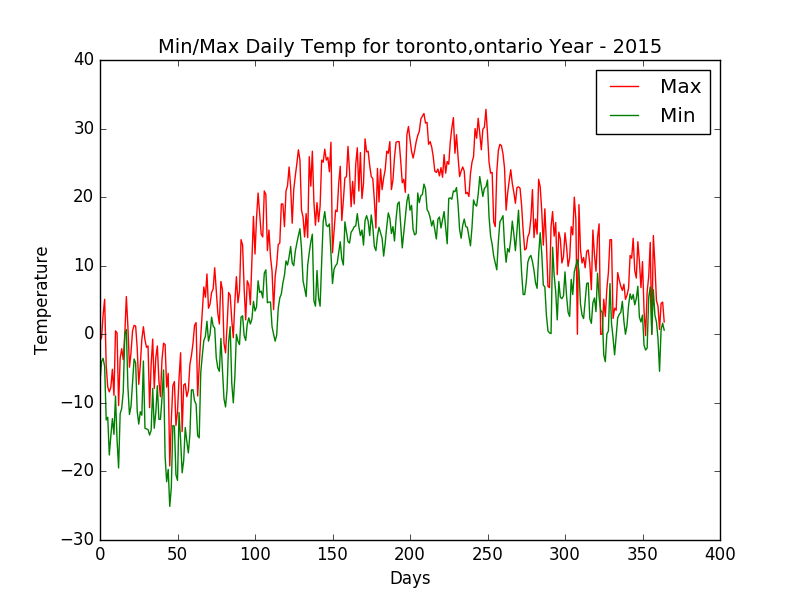
\includegraphics[scale=0.6]{toronto,ontario_MinMax.png}
%\caption{E}
\end{figure}

\begin{figure}
\centering
\includegraphics[scale=0.6]{{"vancouver,british columbia_MinMax"}.png}
%\caption{F}
\end{figure}


\section{Question 3}
Write a command line program that takes arguments\\
In the GDD calculation part, we have used the package argparse to handle the command line arguments. First, we set the csv argument which completes file path of cities file. Second, we set the tbase argument (default = 10) and tupper argument(default = 30) to apply in the GDD calculation.\\
The data needed for GDD calculation are already downloaded and stored in the data folder with their filenames specified in citiex.txt file. In this program, it read these data directly from data folder, do calculation on each file, and store them separately. For the missing information in csv file, we will set the GDD to 0. The GDD calculation equation is below:

In our program, we set the $ T_max$ value to the minimum between tupper and the maximum daily temperature and $ T_base$ to the 10. For example, on 15th, August, 2010 in Vancouver, the maximum temperature is 31.2 Celsius degrees which is more than 30 Celsius degrees, and the minimum temperature is 16.1 Celsius degrees. Hence the GDD equation to $(\frac{30+16.1}{2})-10$  
and the GDD result is $13.05$ .
Finally, we add the new GDD column to the existing data files, which is supposed to prevent creating more files in the project.
In the next part, we are supposed to use the GDD calculation to create plots showing accumulated GDD vs time for selected cities.

\section{Question 4}
Create plots showing accumulated GDD vs time for selected cities.\\
Using the calculation of GDD, the data for the calculation is retrieved from the data folder with their respective filenames specified in cities.txt file. It calculates on each of the file, and plots them separately showing the cumulative GDD vs period for each cities. A loop is written to calculate the cumulative GDD for different years. 
\begin{figure}
\centering
\includegraphics[scale=0.6]{{"st. john's,newfoundland_GddPlot"}.png}
%\caption{A}
\label{fig:gbm}
\end{figure}

\begin{figure}
\centering
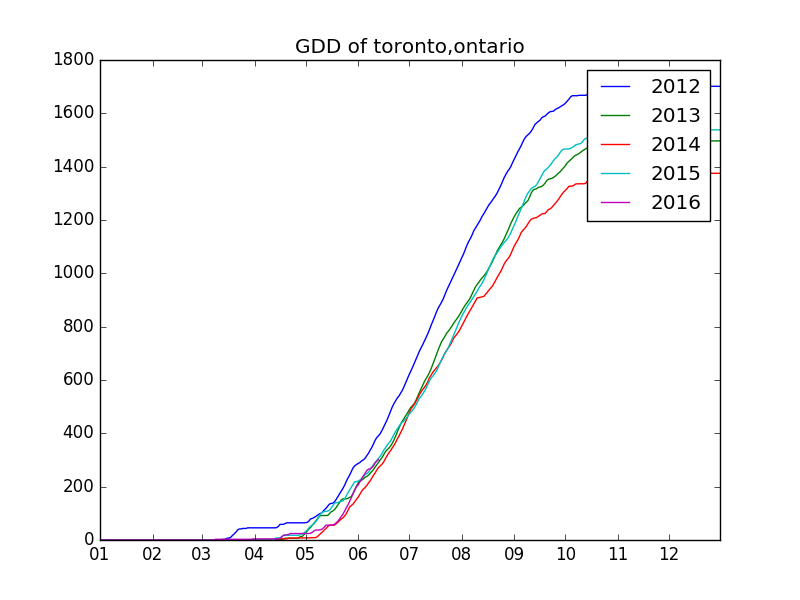
\includegraphics[scale=0.6]{toronto,ontario_GddPlot.png}
%\caption{B}
\label{fig:gbm}
\end{figure}

\begin{figure}
\centering
\includegraphics[scale=0.6]{{"vancouver,british columbia_GddPlot"}.png}
%\caption{C}
\end{figure}

\section{Question 5}
\section{Question 6}
\section{Question 7}
\section{Question 8}
\section{Question 9}
\section{Question 10}
\section{Question 1 optional}
\section{Question 2 optional GDD\_map\_Canada.py}
This code plots a graph of Canada showing the accumulated GDD for several cities along a selected year. When calling the GDD\_map\_Canada.py the user has also to insert cities.txt and the year of interest. GDD\_map\_Canada.py is set to read the files available into the folder named data and the file cities.txt. From cities.txt it is read the cities names and coordinates, in order to plot them in the proper location onto the map of Canada. From the files in the data folder it is used the GDD contained in it and the respective years. \\
The code then assigns different colors for accumulated GDD values for each city according to a scale (red for GDD lower than 510, yellow for GDD lower than 900 and green for GDD higher than 900). Finally, it is plotted a map of Canada in which each city is shown as a dot colored according to the accumulated GDD for that year.
\begin{figure}
\centering
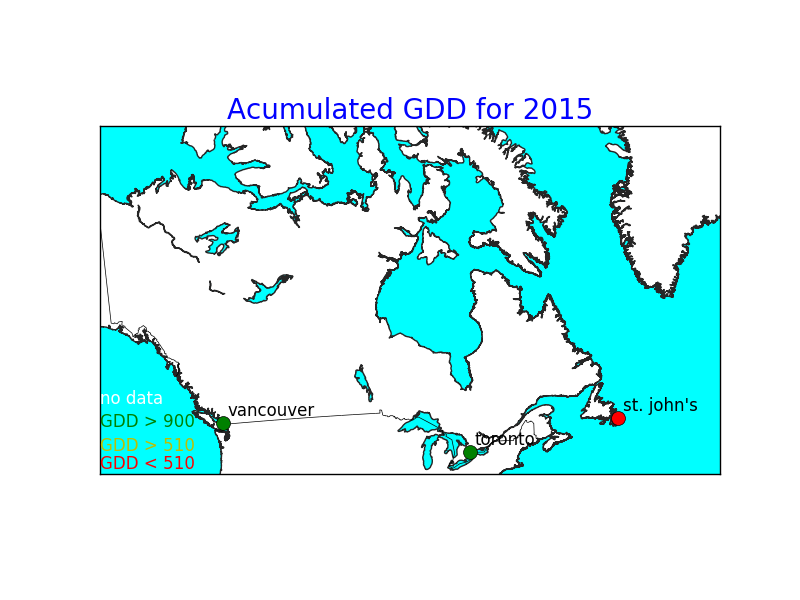
\includegraphics[scale=0.6]{GDDMap_2015.png}
%\caption{F}
\end{figure}
\newpage
\section{Question 3 optional}

From the GDD equation, 
\begin{equation}
\textrm{GDD} = \left(\frac{T_{max} + T_{min}}{2}\right) - T_{base}
\label{eqn:gdd}
\end{equation}
it is obvious that GDD changes with different base temperature. The base temperature is the temperature where the plant growth is 0. The lower the base temperature is, the more GDD is accumulated. Setting base temperature at 10 degree, 11 degree, 12 degree, 13 degree, 14 degree and 15 degree respectively, a graph for accumulated GDD of Toronto, Ontario is displayed in the following graph.\\
\begin{figure}
\centering
\includegraphics[scale=0.6]{{"toronto,ontario_Tbase_GddPlot"}.png}
%\caption{C}
\end{figure}

It can be seen from October to May, no GDD is accumulated because the average temperature is lower than base temperature. From the middle of May, GDD starts to be accumulated, and the lower the base temperature is, the faster the GDD is accumulated.
\begin{figure}
\centering
\includegraphics[scale=0.6]{{"st. john's,newfoundland_Tbase_GddPlot"}.png}
%\caption{C}
\end{figure}

\begin{figure}
\centering
\includegraphics[scale=0.6]{{"vancouver,british columbia_Tbase_GddPlot"}.png}
%\caption{C}
\end{figure}

%\includegraphics{plot00.png}
%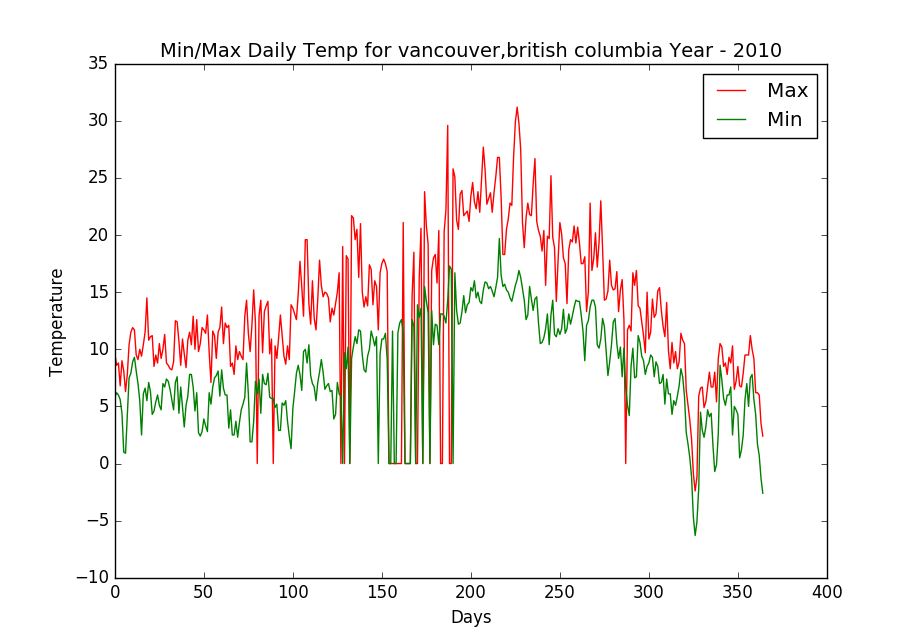
\includegraphics{Plot01.png}
%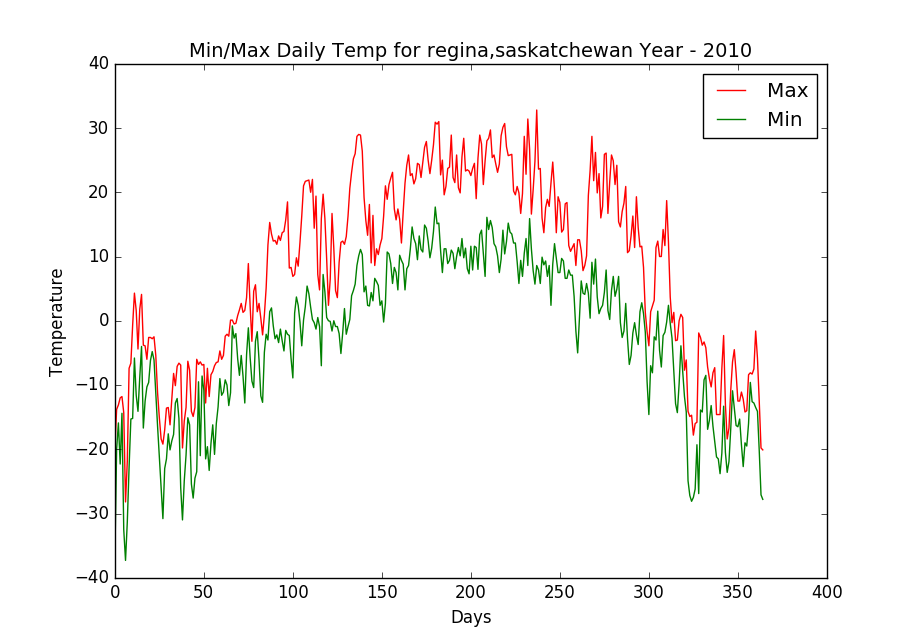
\includegraphics{Plot02.png}
%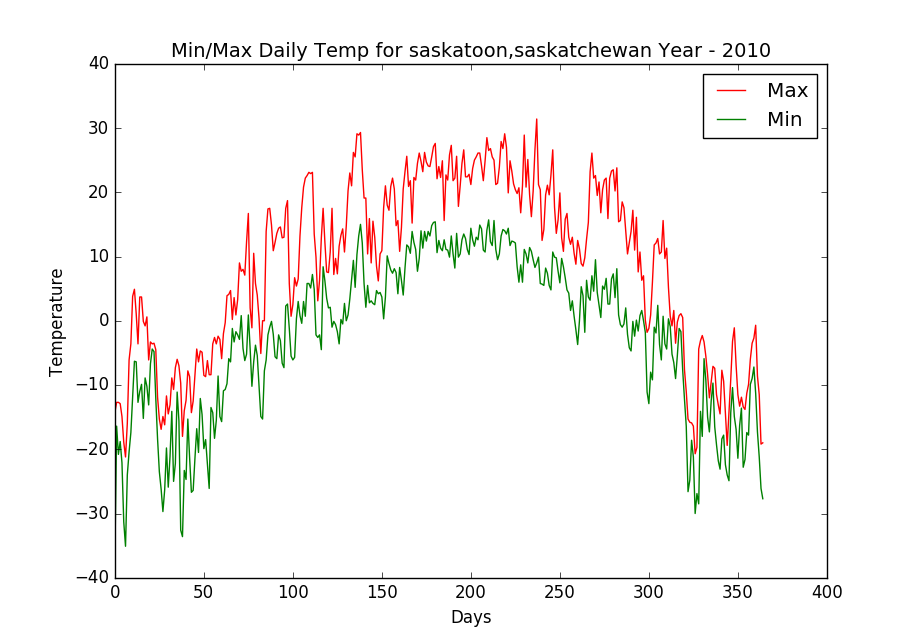
\includegraphics{Plot03.png}
%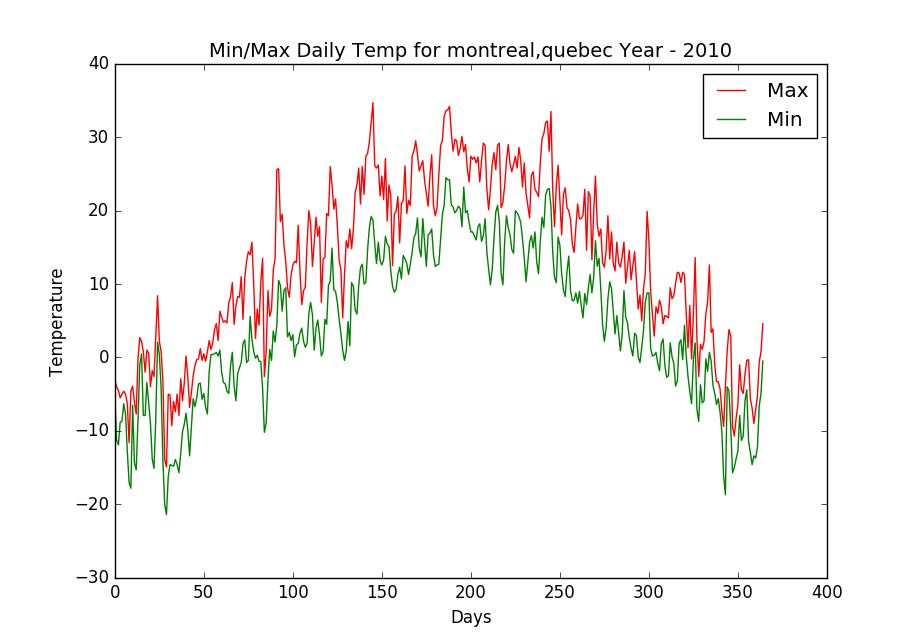
\includegraphics{Plot04.png}
%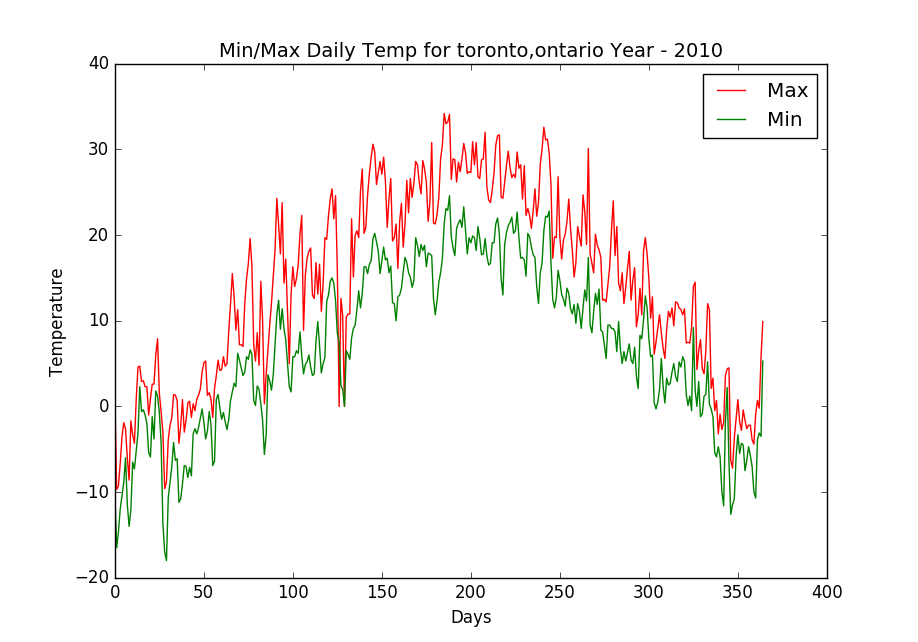
\includegraphics{Plot05.png}
\section{Discussion}
\section{Conclusion}
\newpage
\end{document}
